\documentclass[9pt,conference]{IEEEtran}
\usepackage[nomarkers]{endfloat}
\usepackage[cmex10]{amsmath}
\usepackage[utf8]{inputenc}
\usepackage{filecontents}
\usepackage{lipsum}
\usepackage{graphicx}
\usepackage{rotating}
\usepackage{multirow}
\usepackage{array}

\begin{filecontents*}{informe.bib}
@electronic{refvrp,
  author        = {Wikipedia},
  title         = {VRP brief},
  url           = {http://en.wikipedia.org/wiki/Vehicle_routing_problem},
  year          = {2015}
}
@electronic{refwmaker,
  author        = {Daniel W. Dyer},
  title         = {Referencia Watchmaker},
  url           = {http://watchmaker.uncommons.org},
  year          = {2006}
}
\end{filecontents*}

\begin{document}

%-------- Metadata -------- 
	\title{Informe Proyecto parte 1}
	\markboth{Algoritmos Evolutivos 2015}{Shell \MakeLowercase{\textit{et al.}}: A Novel Tin Can Link}
	\author{
		\IEEEauthorblockN{Gonzalo Torterolo}
		\IEEEauthorblockA{
			Facultad de ingenier\'ia\\
			UDELAR\\
			Montevideo, Uruguay\\
			Email: gonzalo.torterolo@fing.edu.uy
		}
		\and
		\IEEEauthorblockN{Gisel Cincunegui}
		\IEEEauthorblockA{
			Facultad de ingenier\'ia\\
			UDELAR\\
			Montevideo, Uruguay\\
			Email: gisel.cincunegui@fing.edu.uy
		}
	}



% ------- Contenido -------
	\maketitle

	\begin{abstract}
	En esta primer entrega se presenta el problema a solucionar en el correr del proyecto, las principales estrategias de resolución, y los principales focos del estudio experimental.
	En la próxima entrega se intentan aplicar las estrategias planteadas para la resolución práctica del problema. Al final del proyecto se espera lograr una aplicación que logre con recursos computacionales no demasiados elevados y en un tiempo razonable resolver una instancia real o al menos verosímil del problema, junto con un set de datos estadísticos experimentales.
	\end{abstract}
	\begin{IEEEkeywords}
	GA, VRP, TSP, Rescheduling, Crowding, GoogleMaps, watchmaker, java 
	\end{IEEEkeywords}

	\section{Introducción}

	El escenario del problema en cuestión puede enunciarse de la manera siguiente:
	\"Dado un conjunto de pedidos a resolver sobre un mapa, y un conjunto de mandaderos que resuelven los pedidos, se desea encontrar un recorrido para cada mandadero partiendo de un punto inicial, de manera que se resuelvan todos en el menor tiempo posible. A medida que pasa el tiempo y se resuelven pedidos también van llegando nuevos.\"

	El problema puede mapearse a una variante del problema de ruteo de vehiculos, una generalización de TSP \cite{refvrp}, donde además se agrega que el la instancia del problema varíe con el tiempo a medida que llegan nuevos pedidos y se resuelven otros, característica a la que se llama rescheduling de recorridos

	La motivación de este problema es realizar una aplicación móvil/web que permita a un conjunto de personas coordinar sus recorridos de manera eficiente. Esto comprende el agregar/quitar pedidos, ó agregar/quitar mandaderos.

	\section{Análisis}

	\subsection{Variables de entrada}

	Considerando el enunciado inicial del problema se define:

	\begin{enumerate}
		\item N
		Cantidad de puntos en el mapa.
		
		\item M
		Cantidad de mandaderos asignados al problema.
		
		\item Mapa
		Es el conjunto de puntos pi con 0 < i <= N
		
		\item Dist
		La distancia en el mapa del problema, que es una función Dist(x,y) que para dos puntos x,y retorna su distancia en tiempo (es la distancia en tiempo). Todos los pedidos deben ser realizables, por lo que la distancia entre cualquier par de puntos debe ser finita.
		
		\item ColaPendientes
		La lista global de pedidos pendientes a resolver.

		\item Tasa de arribos T
		Es el tiempo cada cuanto se agrega un nuevo pedido a la cola de pendientes. Los puntos del pedido se generan aleatoriamente según una distribución propia del problema.

		\item Punto de origen O
		Representa la ubicación del local a donde se va comenzar el recorrido.
		
		\item R_i 0<i<=M
		Es el recorrido para el mandadero i, una tupla ordenada de puntos del mapa cumpliendo que no tiene puntos en común con ningún otro Xj salvo por el origen.

		\item R
		Es el conjunto de todos los recorridos.

	\end{enumerate}

	El problema busca optimizar el tiempo transcurrido en los recorridos R_i entre todas las instancias R posibles, esto es, intenta minimizar la función objetivo

	%ToDo !!

	TotTime(R) = max 0 <= i < M (Tiempo(R_i))
	Tiempo(R_n) = sum(Dist(p_{i-1}, p_i))

		% \begin{itemize}
		% 	\item Item 1
		% 	\item Item 2
		% \end{itemize}


	\section{Análisis}

	\subsection{Literatura y trabajos previos}

		No se conocen para el proyecto en particular, si para variantes similares. Existe un estudio para un problema simple de VPR que incluye además capacidades y costos aunque no rescheduling (ver http://citeseerx.ist.psu.edu/viewdoc/download?doi=10.1.1.3.7230&rep=rep1&type=pdf), que propone la utilización de una técnica similar al crowding para mantener la diversidad de la población, a partir del mismo se decide utilizar crowding en el algoritmo.


	\subsection{Técnicas a utilizar}

		La utilización de AG parece adecuada para abordar el problema planteado, por las siguientes razones:
			Interesa tener un buen tiempo de respuesta y retornar soluciones de calidad relativamente buena en tiempos cortos de ejecución, los AG al ser técnicas metaheurísticas suelen funcionar más rápido que métodos exactos, sobre todo en problemas NP, como es el presentado.
			Los AG son buenos para problemas combinatorios, pues tienen una formulación algorítmica natural.
			No se suele conocer muchas particularidades 

		Se ha optado por utilizar modelo de islas con la intención de distribuir el cómputo del algoritmo. Esta arquitectura permite paralelizar el cómputo, haciéndola más escalable. Dada esta realidad, puede interesar estudiar el comportamiento de aumentar el tamaño de la población a medida que se incorporan nuevos mandaderos, pues cada uno dispone de un celular que puede aportar en el cómputo. Los parámetros adecuados se estudian en la configuración paramétrica de cada instancia. La migración se realizará de manera asincrónica.

		Codificación
			Se codifican los recorridos de todos los mandaderos utilizando una permutación de puntos del mapa, separando el recorrido de cada mandadero por un separador S, habiendo M-1 separadores.
			R = <R_{i_1}, S, R_{i_2}, ..., S, R_{i_M}>
			Siendo la concatenación de R_i una permutación de todos los puntos del mapa.

		Población inicial
			Se piensa que utilizar alguna heurística como greedy para inicializar la población podría afectar la diversidad, por lo que una inicialización aleatoria parece lo más adecuado.

		Fitness
			El fitness sugerido en una función de minimización es sencillamente la función objetivo:
			Fitness(R) = TotTime(R)

		Operadores evolutivos
			Mutación
				Para la mutación se utiliza sencillamente el intercambio de lugar de un gen del cromosoma. A los fines prácticos su poder disruptivo es tan bueno como cualquier otro, y asegura la obtención de una solución factible. 

			Selección
				La estrategia de selección será por torneo de tamaño M, para evitar calcular el fitness tantas veces, y mu+lamda.

			Cruzamiento
				Se tiene algo muy similar a una permutación, a los fines prácticos se puede adaptar Ordered Crossover para la codificación en cuestión, además en comparación con PMX y CX parece ser menos disruptiva. Este tipo de cruzamiento tiene la propiedad de mantener la cantidad de mandaderos en todo momento, lo que asegura una instancia factible.


	\subsection{Aspectos y consideraciones tecnológicas}

		
		Por su portabilidad al momento de escalar se decide utilizar java como lenguaje de programación.
		
		Por su claridad y sencillez se decide utilizar el framework watchmaker para implementar el AG.
		
		Son muchas las librerías para el manejo de mapas y datos geográficos (algunas investigadas son geotools http://www.geotools.org/ y KML), y muchas son también las fuentes desde donde obtener modelos geográficos realistas/reales (se pueden citar GoogleMaps, datos abiertos de montevideo y OpenStreetMap). La más prometedora ha sido Google DistanceMatrixAPI (https://developers.google.com/maps/documentation/distancematrix/?hl=es-g) y DirectionAPI (https://developers.google.com/maps/documentation/directions/?hl=es-gt), las mismas permiten dar la el tiempo real de un recorrido entre dos puntos geográficos, considerando la forma de las calles y otras restricciones reales.

		El tiempo es otra dimensión importante a determinar. Se exige la que el algoritmo pueda arrojar soluciones de calidad en tiempos del orden de pocos minutos.

		La principal particularidad del problema implica el rescheduling. Para solucionar el mismo, ante el arribo de un nuevo pedido, se mantiene mantiene la población del calculada hasta el momento pero se le agrega a todos los individuos de la población en una posición aleatoria el nuevo punto del pedido; y ante la asignación de un pedido a un mandadero, se eliminan de todos los individuos de la población el punto del pedido. Luego de esto se deja evolucionar el algoritmo para que se ajuste al cambio.

	% \begin{itemize}
	% 	\item item A.
	% 	\begin{itemize}
	% 		\item Item 1
	% 		\item Item 2
	% 	\end{itemize}
	% 	\item Item B
	% 	\begin{itemize}
	% 		\item Item 1
	% 		\item Item 2
	% 	\end{itemize}
	% \end{itemize}

	\section{Evaluación experimental}

	\subsection{Ajuste y Configuración Paramétrica}

		En la configuración paramétrica se van a probar diversas instancias de ajuste y comparar los resultados en distintos casos. Una vez determinado los mejores parámetros se inicia la evaluación experimental.
		Las instancias a utilizar serán generadas a partir de una selección de puntos de un mapa real, y la distribución a tomar de estos se generarán a partir de información de densidad de población ó cantidad de puntos de interés, etc de cada mapa. Se maneja la posibilidad de usar GooglePlaces como fuente de referencia para las distribución de los puntos.
		
		En resumen, los parámetros a configurar dadas las técnicas antes definidas son:
			Tamaño de población: El tamaño global de la población.
			Mutación: Probabilidad de mutación.
			Reemplazo:
				Crowding: El delta de crowding debe ser determinado.
			Islas:
				Uso de islas.
				Número de islas.
				Número de islas en relación a cantidad de mandaderos.
				Tasa de migración.
				Topología.

	\subsection{Dimensiones del problema}

			En una primer etapa de ajustes deberá importar el rendimiento que alcance el algoritmo, pero su principal objetivo es verificar la correctitud funcional del mismo.
			Al momento de realizar la evaluación experimental se espera poder manejar instancias de dimensiones realistas.

			Haciendo un análisis de las variables de decisión, se enfocará el estudio sobre los casos particulares donde se tiene:
				Una cantidad reducida de mandaderos en comparación a los puntos del mapa, pues el caso contrario tiende a ser cada vez más sencillo y algoritmos greedy alcanzan el óptimo mejor.
				También a medida que la tasa de arribo de nuevos pedidos se hace más grande, el problema se asemeja a un VPR clásico, no es el principal interés resolver este caso, pero puede ser de utilidad a modo de contrastar la calidad del algoritmo con implementaciones conocidas. Del mismo modo a medida que se reduce la cantidad de mandaderos a 1 el problema se reduce a un TSP clásico.

	\subsection{Pruebas}

		El proceso de evaluación experimental comprenderá:
			Análisis comparativo de calidad de solución con un algoritmo greedy trivial.
			Análisis comparativo del mismo algoritmo usando islas y sin usar islas.
				En distintos entornos de ejecución paralelo VS secuencial (Cluster VS Máquinas domésticas).
			Análisis de evolución del sistema. Tiempo VS mejora de la función de fitness.
			Análisis de sensibilidad a las entradas:
				Se estudiará cuanto tarda en estabilizarse la solución y una vez que el sistema entre en régimen como varía la calidad de la solución obtenida a lo largo del tiempo.
				El mismo procedimiento se piensa realizar variando cantidad de mandaderos y la tasa de arribo de pedidos.



	% \section{Análisis}

	% \subsection{Ajuste y Configuración Paramétrica}


		% $$X_i,C_i$$\\ son la cantidad de aperitivos, costo de aperitivo para el tipo $i$ respectivamente\\
		% $$N,O$$\\ la dimensi\'on del problema y costo objetivo respectivamente\\

	% \begin{enumerate}
	% 	\item item B.
	% 	Lorem ipsum

	% 	\item alternat

	% 		\begin{equation}
	% 		\label{eqn_tope_req}
	% 		M_i = \lceil \frac{N}{C_i} \rceil
	% 		\end{equation}


	% 	\item item C
	% 		Lorem lorem ipsum ipsum amoret amoret
	% 		\[ v = |\sum\limits_{i=0}^{N} (C_i X_i) - O| \]
	% 		Lorem lorem ipsum ipsum amoret amoret.
	% 		\[ X_i = (X_i + rand(0,M_i)) \% M_i \]

	% \end{enumerate}

	% \subsection{some subsec}

	% \begin{itemize}
	% 	\item some item:
	% 	En ecuaciones ver \ref{eqn_tot_gain} y \ref{eqn_tot_peso}:
		
	% 	\begin{equation}
	% 		\label{eqn_tot_gain}
	% 		G_{tot} = \sum\limits_{i=0}^{n} g_{i}x_{i}
	% 	\end{equation}

	% 	\begin{equation}
	% 		\label{eqn_tot_peso}
	% 		P_{tot} = \sum\limits_{i=0}^{n} p_{i}x_{i} < W
	% 	\end{equation}

	% \end{itemize}	
	% \begin{enumerate}
	% 	\item Funcion de fitness:\\
	% 	\begin{itemize}

	% 		\item Funcion sin penalizacion:\\

	% 		\begin{IEEEeqnarray}[\setlength{\nulldelimiterspace}{0pt}]{rl,s}&G_{tot},&for $P_{tot} \le W$\IEEEyesnumber\IEEEyessubnumber\\*
	% 		[-0.625\normalbaselineskip]
	% 		\smash{fitness(x)=\left\{\IEEEstrut[3\jot][3\jot]\right.}&&
	% 		\nonumber\\*[-0.625\normalbaselineskip]
	% 		&G_{tot}-(\frac{2 G_{tot} (k-p)}{k}),&for $P_{tot} > W$\IEEEyessubnumber
	% 		\end{IEEEeqnarray}

	% 		\item Funcion sin penalizacion:\\

	% 	\end{itemize}	

	% 	\item Condici\'on de parada:
	% 		10000 generaciones.
	% \end{enumerate}

	% \section{Ejecuciones}
	% Lorem ipsum

% 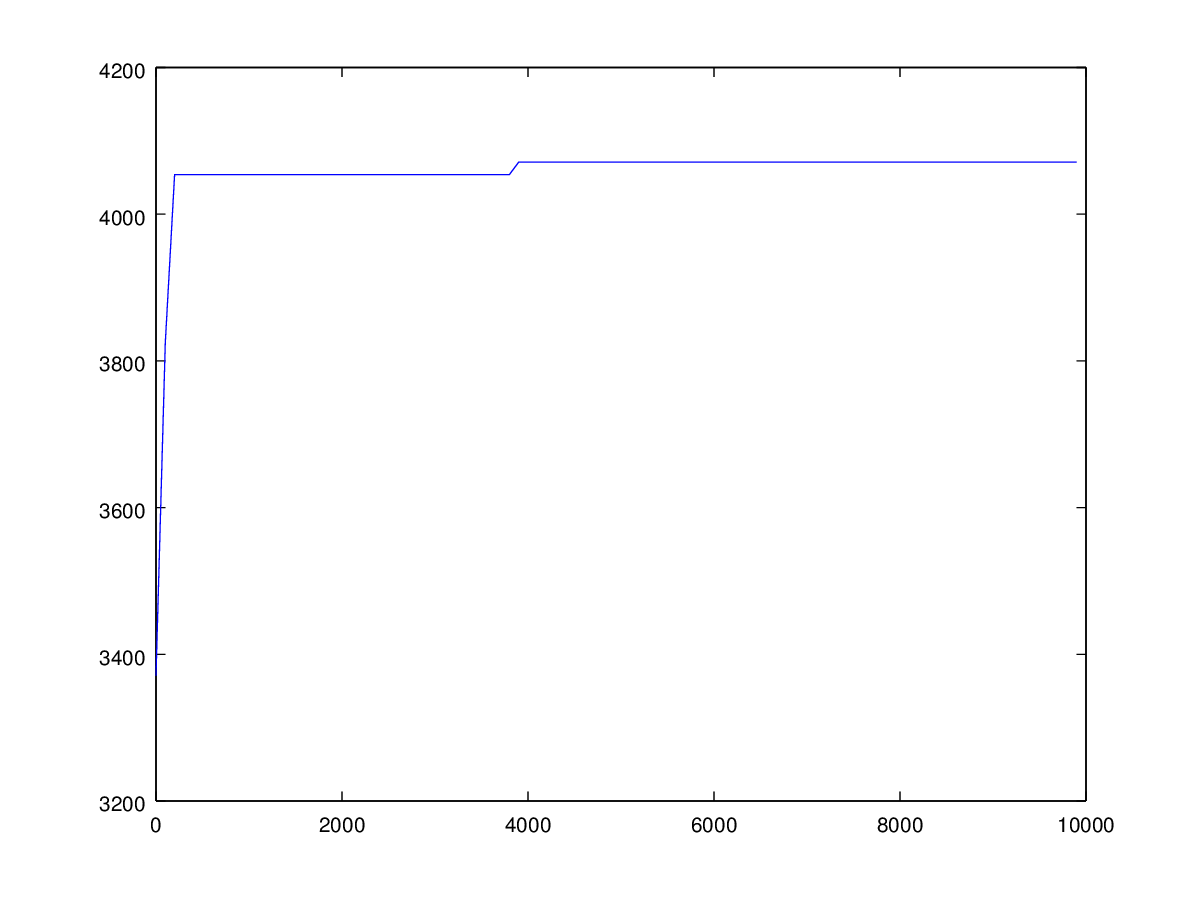
\includegraphics[width=0.5\textwidth]{images/graf_test_in.png}

% 	\section{Conclusi\'on}
% 	Lorem Ipsum amoret
% % ------ Final ------

% 	\bibliographystyle{IEEEtran}
% 	\bibliography{informe.bib}{}

\end{document}